\chapter{Implementacja} \label{chap:implementation}

\section{Opis modelu danych do reprezentacji skrzyżowań}

Drogi są reprezentowane w sposób dyskretny. Każda droga zaczyna się w pozycji 1 i rośnie wraz z jej rozmiarem. 
\newline
\newline
Samochody mogą poruszać się w następujących kierunkach:
\newline
- z północy na południe
\newline
- z południa na północ
\newline
- ze wschodu na zachód
\newline
- z zachodu na wschód
\newline
\newline
Powyższe ogarniczenie nie wpływa na algorytm lub wyniki. Dodanie funkcjonalności wymagałoby dodania możliwości zmiany numeru drogi przez samochód, co nie wpływa na liczbę stanów, a co za tym idzie długości wykonywania algorytmu.
\newline
\newline
Droga jest reprezentowana poprzez następujące dane:
\newline
- unikatowy numer drogi
\newline
- rozmiar drogi
\newline
- informacja o przecięciach z innymi drogami
\newline
- kierunek w którym samochód się porusza na drodze (z północy na południe, czy z południa na północ lub z zachodu na wschód czy ze wschodu na zachód)
\newline
\newline
Samochody na drogach opisują następujące dane:
\newline
- unikatowy numer samochodu
\newline
- unikatowy numer drogi, na której pojazd się znajduje
\newline
- numer pozycji na drodze, na której samochód się znajduje
\newline
- prędkość początkowa
\newline
- numer pozycji docelowej na drodze - punkt za ostatnim skrzyżowaniem
\newline
\newline
Samochody poruszają się po drogach w krokach czasowych. Prędkość samochodu wyrażana jest w liczbie odcinków drogi w jednym kroku czasowym.
\newline
\newline
W Systemie można wybrać maksymalne przyspieszenia ujemne oraz dodatnie samochodów z następujących możliwości \{-2, -1, 0, 1, 2\}. Oznacza to, że w następnym stanie pojazd może przyspieszyć o 1 lub 2 odcinki drogi na jeden krok czasowy. Dla wartości 0 pojazd utrzymuje swoją prędkość. Dla wartości ujemnych pojazd zwalnia o 1 lub 2 odcinki drogi na jeden kroku czasowym. Ilość możliwych dla samochodu przyspieszeń znacznie wpływa na złożoność czasową algorytmu, z tego względu, że wraz ze wzrostem ilośći możliwych przyspieszeń rośnie ilość możliwość stanów sąsiednich dla samochodu, przez które algorytm musi przejść.        
\newline
\newline
Do modelu przekazać należy także maksymalną prędkość, którą wszystkie samochody mogą osiągnąć oraz parametr prędkości, czyli liczba pozyji będąca dystansem trzymanym między pojazdami.

\section{Zmodyfikowany algorytm A*}

Zaprezentowany w tej pracy zmodyfikowanym algorytmu A* jest oparty na stanach, gdzie pojedyńczym stanem jest rozłożenie samochodów na drogach wraz z ich prędkościami.
\newline
\newline
Algorytm zaczynając od zadanego stanu początkowego analizuje możliwe stany sąsiednie i wybiera optymalną ścieżkę kierując się funkcją heurystyki. Ścieżka prowadzi do określonego celu.
\newline
\newline
W przypadku opracowanego rozwiązania, celem jest przekroczenie przez wszystkie samochody ostatniego skrzyżowania na drogach, na których się znajdują.
\newline
\newline
Zrealizowany Algorytm A* jest generyczny. Do algorytmu przekazujemy klasę reprezentującą dowolny stan. Klasa musi implementować metodę 'neighbours', która zwraca stany sąsiednie dla danej instancji stanu.
\newline
\newline
Do algorytmu przekazywana jest także funkcja heurystyki, zależna od danych danego stanu.

\section{Stan w opracowanym rozwiązaniu dla algorytmu A*}

Stan w modyfikacji algorytmu A* przedstawionej w tej pracy opisuje stan wszystkich samochodów na skrzyżowaniach wraz z ich prędkościami.
\newline
\newline
Zgodnie z wcześniej generycznością wierzchołek jest obiektem klasy, który implementuje metodę 'neighbours'. Metoda generuje wszystkie stany sąsiednie dla aktualnego stanu. Dla przykładu, dla ustawień przyspieszeń \{-2, -1, 0, 1, 2\}, dla każdego z aut na skrzyżowaniu generowane są stany z jego prędkością dodając wartości przyspieszeń. Pomijane są stany, w których prędkość samochodu byłaby ujemna.
\newline
\newline
Przykładowo jest pojazd z prędkością 1 pozycja na krok czasowy znajdujący się na 1 pozycji na drodze numer jeden. Dla pojazdu rozpatrywane są następujące stany:
\newline
1) Dodając przyspieszenie o wartości 0: 2 pozycja na drodze numer jeden z prędkością 1
\newline
2) Dodając przyspieszenie o wartości 1: 3 pozycja na drodze numer jeden z prędkością 2
\newline
3) Dodając przyspieszenie o wartości 2: 4 pozycja na drodze numer jeden z prędkością 3
\newline
4) Dodając przyspieszenie o wartości -1: 1 pozycja na drodze numer jeden z prędkością 0
\newline
5) Dodając przyspieszenie o wartości -2: Stan jest eliminowany, ponieważ prędkość byłaby ujemna
\newline
\newline
Dodatkowo w przypadku ustawienia maksymalnej prędkości równej 2 pozycje na jeden krok czasowy - możliwość nr 3) także zostałaby wyeliminowana.
\newline
\newline
W metodzie usuwane są także stany powodujące kolizje, co będzie opisane w następnym rozdziale.

\section{Unikanie kolizji}

Koniecznym elementem w planowaniu ruchu jest unikanie kolizji.
\newline
\newline
Unikanie kolizji zostało podzielone na dwa etapy
\newline
- Unikanie kolizji aut poruszających się po tym samym pasie
\newline
- Unikanie kolizji na skrzyżowaniach
\newline
\newline
Impementacja unikania kolizji pojazdów na tym samym pasie polega na policzeniu obszarów dla samochodów znajdujących się na tym samym pasie, który będą one obejmowały w jednym kroku czasowym wraz z uwzględnieniem parametru bezpieczeństwa.
\newline
\newline
Jeżeli obszary dwóch samochdów na jednym pasie pokrywają się - taki stan jest usuwany i wówczas metoda 'neighbours' nie zwróci go jako stanu sąsiedniego.
\newline
\newline
Na rysunku \ref{collision-avoidance-lane} przedstawiony jest przykładu unikania kolizji dla samochodów poruszających się jednym pasem. Przykład przedstawiony jest z parametrem bezpieczeństwa równym jeden.
\newline
Jak widać samochody, mając przed sobą inny pojazd, czekają aż będzie dla nich miejsce.
\begin{figure}
    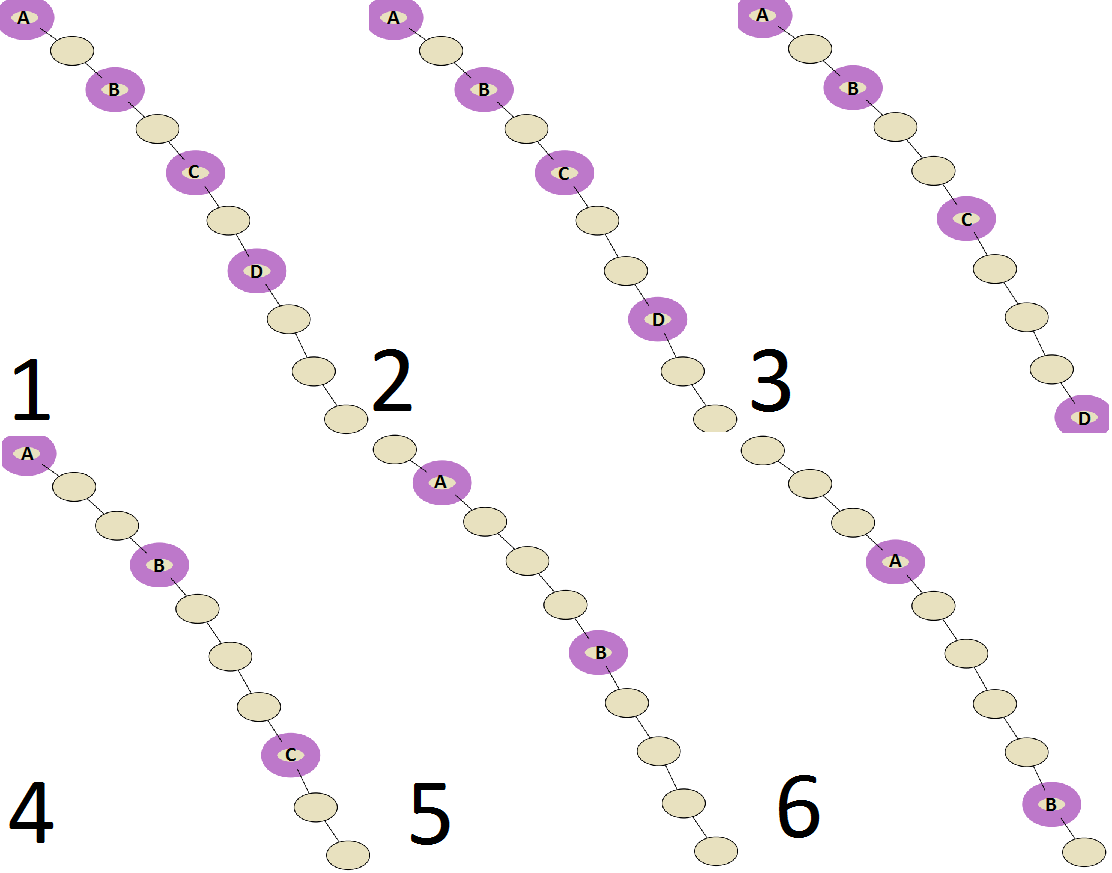
\includegraphics[width=1.0\textwidth]{collision-avoidance-lane.png}
  \caption{Unikani kolizji na pasie}
  \label{collision-avoidance-lane}
\end{figure}
\newpage
Unikanie kolizji na skrzyżowaniach polega na eliminacji stanów, w których conajmniej dwa auta przekroczyły w jednym kroku czasowym to samo skrzyżowanie. Metoda 'neighbours' także nie zwróci takich stanów.
\newline
\newline
Na rysunku \ref{collision-avoidance-crossroads} przedstawiony jest przykładu unikania kolizji dla dwóch samochodów na prostym skrzyżowaniu. Samochód z numerem jeden przyspieszył o dwie jedostki i zmienił pozycję o dwie jednostki do przodu. Samochód z numerem dwa przyspieszył natomiast o jedną jednostkę i zmienił pozycję o jedną jednostkę do przodu w celu uniknięcia kolizji.
\newline
\newline
W algorytmie usunięty został stan, w którym oba pojazdy przyspieszyły o dwie jednostki. Został natomiast wybrany stan gdzie jeden z samochodów przyspieszył o dwie jednostki, a drugi o jedną jednostką, ponieważ prowadzi to, do najszybszego opuszczenia przez pojazdy skrzyżowania.
\begin{figure}
    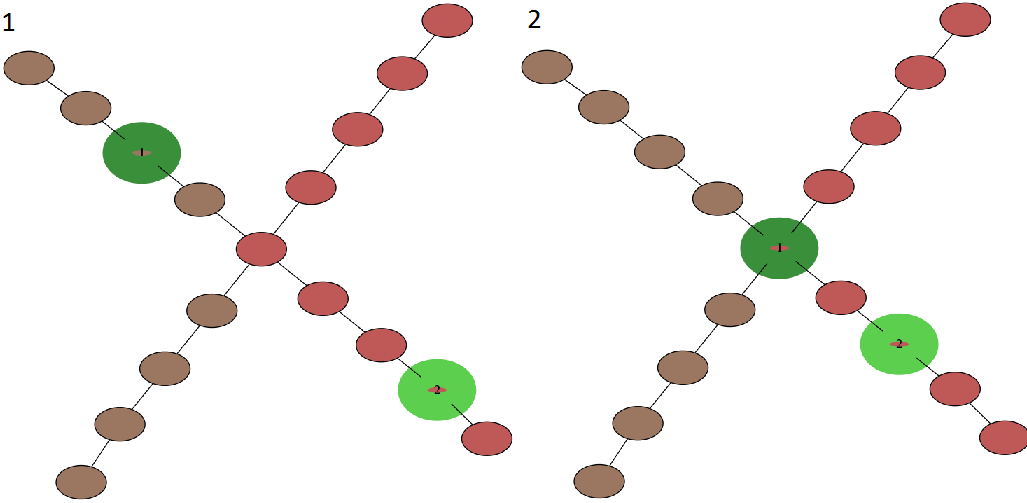
\includegraphics[width=1.0\textwidth]{collision-avoidance-crossroads.png}
  \caption{Unikanie kolizji na skrzyżowaniu}
  \label{collision-avoidance-crossroads}
\end{figure}
\newpage

\section{Funkcja heurystyki}

Funkcja heurystyki dla algorytmu A* jest to suma kroków czasowych, po których wszystkie auta przekroczą ostatnie skrzyżowanie - czyli osiągną cel. Funkcja liczona jest, przy założeniu, że wszystkie samochody maksymalnie przyspieszają.

\section{Reprezentacja graficzna wyników}

W celu graficznej reprezentacji wyników zaimplementowany został moduł graficzny.
\newline
\newline
Działanie modułu graficznego oparte jest na rysowaniu grafów z wykorzystaniem biblioteki Graphviz oraz jej implementacji w języku Ruby.
\newline
\newline
Skrzyżowanie jest reprezentowane za pomocą grafu. Wierzchołkami grafu są poszczególne odcinki dróg. Krawędziami grafu są połączenia pomiędzy odcinkami.
\newline
\newline
Każda droga jest oznaczona innym kolorem.
\newline
\newline
Samochody poruszające się po tej samej drodze są zaznaczone grubszym obwodem oraz mają ten sam kolor. Samochody można rozróżnić poprzez unikatowy numer na nich napisany.
\newline
\newline
Kolejne kroki czasowe reprezentowane są poprzez następne grafy z kolejnymi ułożeniami samochodów.
\newline
\newline
Ostatnim elementem modułu graficznego jest stworzenie GIFa z następujących po sobie grafów.
\newline
\newline
%Poniżej na rysunkach \ref{1-traffic} - \ref{12-traffic} jest przedstawione zostało rozwiązanie dla dwunastu pojazdów na skrzyżowaniu ośmiu dróg.
\newline
%Jak widać na rysunku \ref{12-traffic} po dwunastym kroku czasowym wszystkie samochody opóściły skrzyżowanie.
